
\subsection{Introduction}
Synthetic data can be defined as data that has no connection with a real-world phenomenon or event. It did not originate from a process in the real world, but rather a synthetic one. The idea is that synthetic data can have similar properties with real data, without needing to have an independent process for its generation.
Synthetic data has been used over the years for several usages, but in healthcare is still not very used. However, this scenario seems to be changing. It can be used for several use cases namely \cite{synthetic-data-usage}; i) Software testing, ii) educational purposes, iii) \ac{ml}, iv) regulatory, v) retention, vi) secondary and vii) enhanced privacy.

Software testing relates to using synthetic data to create use cases for software testing. This can be used for the development or pre-production stages for example. Often the data needed is not available on-demand and a synthetic generator of reliable data could be useful. Educational purposes relate to, at least, two different scenarios. One is for onboarding of employees \cite{synthetic-data-usage}, the other is related to healthcare students for using health information systems and creating mechanisms for providing reliable data on-demand.
\ac{ml} is one of the areas where synthetic data has more widespread usage, where data augmentation through data synthesis is already common. It can be used for class imbalance, sample-size boosting, or machine-learning algorithm testing. Regulatory purposes could be important as well, with the rise of \ac{ai} as medical device systems and synthetic data could be used to properly evaluate these systems under controlled environments. Retention can be an important case for synthetic data as well, since personal data must not be kept more than it would be necessary. Synthetic data generators can be of use, where the original data can be deleted and a generator kept for further usage, given that the privacy mechanisms are properly employed. Secondary uses relate to using synthetic data to share data with academia or industry. Simulacrum \cite{simulacrum} is a nice example of how the NHS uses these mechanisms to help scientists get a better grasp of data before having to fill in documentation to query the real data. The same occurs for \ac{IKNL}, which has a synthetic version of the cancer registry for scientific purposes \cite{synthetic_2} and the \ac{MHRA} that uses synthetic data as well for its CPRD real-word evidence \cite{mhra_cprd}.

Finally, an aspect that is underlying all these applications is the promise that synthetic data can be used to improve privacy. Even though specially tweaked data generators can be used to create more privacy-aware datasets, it will be inherently always at the cost of some utility \cite{stadler_synthetic_2020}. So, even though synthetic data is not the silver bullet as primarily thought, synthetic data generation can be undeniably used to help create more private data for all the use cases seen above at the cost of its utility. As for proper methods of evaluating security and utility, there are, for now, open research questions. At the present time, it is still complicated to properly assess the utility of the generated data. We have qualitative and quantitative methods. Qualitative methods are related to plots, and quantitative are related to some value that defines an evaluation metric. These quantitative metrics can be applied to equal columns from each data set, pair of columns from each dataset or applied over the whole dataset. As for privacy metrics, the metrics rely on duplicates. Full duplicates or membership inference related. 

So in this paper, we developed a data pipeline for data analysis in order to create a report for providing several metrics for data utility and privacy.


\subsection{Methods}


The pipeline relies on Python and latex for creating the document. It relies also on several packages that implemented methods for evaluating data, namely scipy \cite{scipy}, sdmetrics \cite{sdv} and \textit{scikit-learn} \cite{scikit-learn} and \textit{mlxtend} \cite{mlxtend}. Its basis is related to uploading 2 datasets, and a report in pdf is produced. Being that is based on programmatic code, it can be easily converted into \ac{api}.
The report has a section for dataset description, columns removed due to high-null, and a brief variable overview. Then a null comparison is done by column and dataset. Following this is the utility subsection. Firstly, by visual methodologies: heat maps for the correlation, bar plots for categorical, density plots for continuous, and a pair plot for an overview. As for the quantitative utility evaluation, we divided it column-wise, pair-wise, and table-wise. The first comprehends the \ac{ks} test for continuous and $\chi^2$ test for categorical variables.  Distance metrics were also applied to categorical columns. First, they are transformed into distributions and then distance metrics are applied. The results is a descriptive overview of the distance metrics, having minimum value, average, max value, and standard deviation. The distance metrics selected were \ac{jsd}, \textit{Wasserstein distance}, \textit{Kullback–Leibler divergence}, and entropy.
As for pair-wise metrics, we used a discrete and continuous \textit{Kullblack-Leibler divergence}. In this, two pairs of continuous columns are compared using \textit{Kullback–Leibler divergence}. For this, they are put into bins for further application. The same is applied to categorical columns without binning.
As for table-wise metrics, first, we used likelihood metrics. We fitted several Gaussian Mixture models or \ac{bn} models to the real data and then calculated the likelihood of the synthetic data belonging to the same distribution. The metrics are likelihood for the Gaussian mixture and Bayesian models and log-likelihood for the Bayesian model as well.

\begin{table}[htpb]
    \caption{Metrics Assessed}
    \label{tab:variables}
    \centering
\begin{tabular}{@{}lll@{}}   \toprule
Metric                       & Method       & Context         \\\midrule
Bar Plot                     & visual       & utility         \\ 
KDE Plot                     & visual       & utility         \\ 
Heat-map                     & visual       & utility         \\ 
Pair-plot                    & visual       & utility         \\ 
KS test                      & column-quantitative & utility         \\ 
ChiSquared Test              & column-quantitative & utility         \\ 
Kullback–Leibler divergence  & column-quantitative & utility         \\ 
Jensen-Shannon Divergence    & column-quantitative & utility         \\ 
Wasserstein distance         & column-quantitative & utility         \\ 
Entropy                      & column-quantitative & utility         \\ 
DiscKLD                      & table-quantitative & utility         \\ 
ContinuousKLD                & table-quantitative & utility         \\ 
BNLikelihood                 & table-quantitative & utility         \\ 
BNLogLikelihood              & table-quantitative & utility         \\ 
GMLogLikelihood              & table-quantitative & utility         \\ 
Same dataset ratio           & table-quantitative & utility         \\ 
Support rules                & table-quantitative & utility         \\ 
Different dataset validation & table-quantitative & utility         \\ 
Duplicates                   & quantitative & privacy         \\ 
Duplicate minus 1            & quantitative & privacy         \\ 
Record Linkage             & quantitative & privacy         \\ 
Matrix distance              & quantitative & privacy/utility  \\ 
Cosine distance              & quantitative & privacy/utility \\ 
Euclidean distance           & quantitative & privacy/utility \\ \bottomrule

\end{tabular}
\end{table}


Then we used machine-learning models (linear regression and decision trees) to assess how similar models behave on both datasets. First, we tested on the same dataset in order to compare evaluation metrics. Then we cross-tested, meaning that the training set was drawn from one dataset and the test set was drawn from the second dataset. Finally, data privacy constraints duplicate evaluation, duplicate existence by removal of a single column and a record linkage approach. With the record linkage, we define a record linkage blocking ("age" in the example) and then try to match rows from the synthetic dataset to the real, with varying known attributes. Then matrix, euclidean and cosine distance was also calculated. Even though it is used for privacy evaluation, by definition, we could also use it for utility assessment. For proper assessment, the continuous and categorical variables should be indicated at the start of the code. The metrics are listed in the table \ref{tab:variables}.




%class GMLogLikelihood(SingleTableMetric):
%    """GaussianMixture Single Table metric.
 %   This metric fits multiple GaussianMixture models to the real data and then
  %  evaluates how likely it is that the synthetic data belongs to the same
%    distribution as the real data.


%class BNLikelihood(SingleTableMetric):
%    """BayesianNetwork Likelihood Single Table metric.
%    This metric fits a BayesianNetwork to the real data and then evaluates how
%    likely it is that the synthetic data belongs to the same distribution.
%    The output is the average probability across all the synthetic rows.


%class BNLogLikelihood(BNLikelihood):
%    """BayesianNetwork Log Likelihood Single Table metric.
%    This metric fits a BayesianNetwork to the real data and then evaluates how
%    likely it is that the synthetic data belongs to the same distribution.
%    The output is the average log probability across all the synthetic rows.
    
%CSTest: Chi-Squared test to compare the distributions of two categorical columns.
%KSTest: Kolmogorov-Smirnov test to compare the distributions of two numerical columns %using their empirical CDF.


%
%class ContinuousKLDivergence(ColumnPairsMetric):
%	 """Continuous Kullback–Leibler Divergence based metric.%
	
%	 This approximates the KL divergence by binning the continuous values
%	 to turn them into categorical values and then computing the relative
%	 entropy. Afterwards normalizes the value applying ``1 / (1 + KLD)``.




\subsection{Results}
A trial example of comparing data is available for data in the \ac{uci} repository, namely the heart disease dataset \cite{misc_heart_disease_45}. The synthetic data was created by using the synthpop package \cite{synthpop}. The variables evaluated are listed in table below. The code can be seen in \url{https://github.com/joofio/dataset-comparasion-report}. As an example, the image for visual analysis for categorical (figure \ref{fig:catgorical}) and continuous variables (figure \ref{fig:continuous}).


\begin{figure}[H]
    \centering
    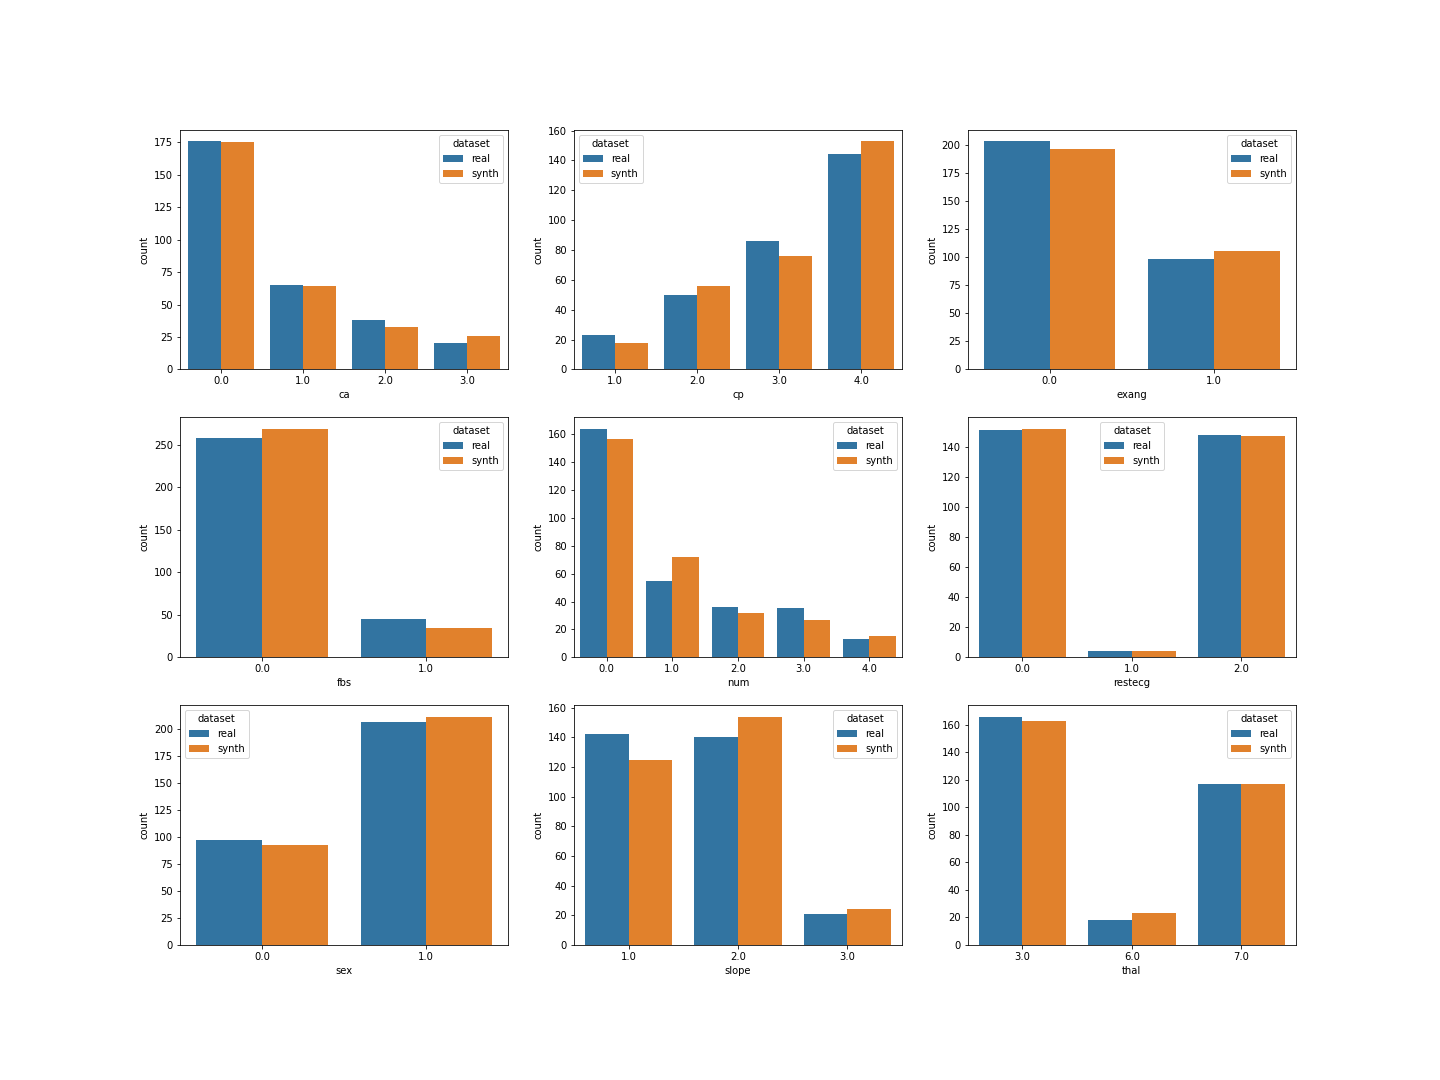
\includegraphics[scale=0.23]{figures/cat.png}
    \caption{Categorical Variables plotted}
    \label{fig:catgorical}
\end{figure}

\begin{figure}[t]
    \centering
    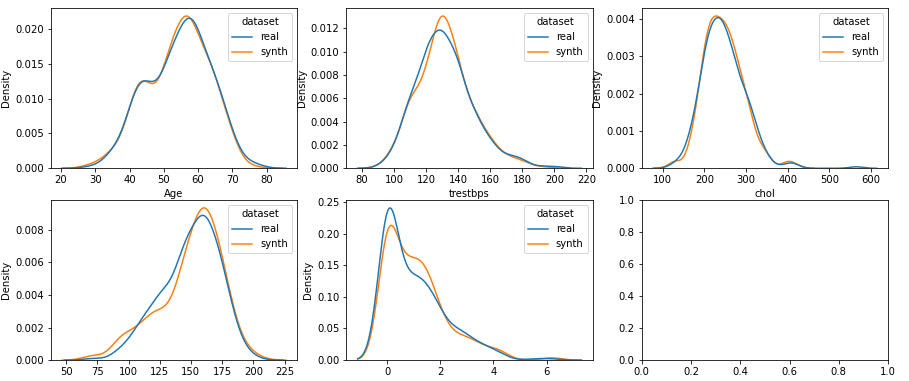
\includegraphics[width=\textwidth]{figures/continuous_plot_0.png}
    \caption{Continuous Variables plotted}
    \label{fig:continuous}
\end{figure}



\subsection{Discussion \& Conclusion}

The data possible to create to evaluate similarities between two datasets is important not only for synthetic vs real datasets. For example, in distributed learning, where different silos exist, with similar or even equal features, a method for evaluating the similarities can be useful for understanding how the populations are similar between them, trying to shed light on the most similarities among them, or different in order to understand the differences in the silos or data acquisition inside them.
Furthermore, the differences can be assessed on a more granular level. The column-wise similarities can be different from the inter-column similarities and this in itself, can be a metric of interest regarding the quality of the synthetic data and its generator.

With this work, we hope to help institutions and academics get access to a benchmark of the datasets provided in order to leverage synthetic data in the healthcare space. Finally, we hope this work helps other researchers reach an evaluation metric that could be a unique and clear response to the question of how similar two datasets are.
